%!TEX root = ../../dokumentation.tex

\textbf{Asynchronous Messaging}

For asynchronous messaging, the technologies RabbitMQ with its supported protocols, \ac{NATS} and Apache Kafka are presented.
RabbitMQ is used as a representative for all technologies that implement \acf{AMQP}, \acf{MQTT} or \acf{STOMP}.
Apache Kafka is a relatively new technology that has attracted much attention.
It was already introduced in the TechnologyRadar in 2016 \cite{ThoughtWorks.01.06.2020} and a new technique \textit{Event streaming as the source of truth} is becoming more and more popular \cite{ThoughtWorks.01.06.2020b}, which fits perfectly with Apache Kafka.
\ac{NATS} is also quite new, but its main focus is on availability, while RabbitMQ and Apache Kafka focus more on consistency.
Therefore, these three technologies represent a wide range of asynchronous messaging systems.

\subsection{RabbitMQ}\label{cha:Technologies:communication:rabbitmq}

RabbitMQ is an implementation of the \acf{AMQP}.
The protocol follows a Publish-Subscribe pattern.
The communication flow of \ac{AMQP} is shown in Figure \ref{img:rabbitmqamqp}.
It is important to note that multiple publishers can publish to the same exchange entity, one exchange entity can route to multiple queues and multiple consumer can listen at one queue.
The routing of an exchange entity can be configured in four different ways.
To explain the different configurations, it is important to note that each message contains a routing key and can contain n-header information.
Both are used by the exchange entities, but in different ways depending on the configuration.
The following list shows the differences between the configurations in terms of how they route a message to an associated queue \cite{RabbitMQ.2020}\cite[p.~26ff.]{SanjayAiyagarietal.2008}.

\begin{itemize}
	\item Direct: (default) Route a message based on its routing key.
	\item Fanout: Copies the message and sends it to each queue, regardless of the message information.
	\item Topic: Works like Fanout, but also uses the routing key. Queues define regular expressions to determine whether a routing key can be associated with that queue.
	\item Header: Ignores the routing key and uses header information to route a message. This is highly configurable by itself.
\end{itemize}

Exchange entities and queues can be defined in advance or by the publisher and consumer.
If they are defined by the publisher or consumer, the required configuration is provided and sent to RabbitMQ.
When connecting to an exchange or queue its configuration must be provided.
If it doesn't exist, then a new one is created.
If it does exist and the configuration matches the existing one, then a connection is established.
If the provided configuration does not match the configuration of the existing exchange or queue, an error is thrown.
Publisher define exchanges and consumer define queues.
When defining a queue, a binding is required that connects the queue to an exchange entity.
The binding can consist of a routing key (direct exchange), regular expression (topic exchange) or nothing (fanout exchange and header exchange) \cite{RabbitMQ.2020}.

It is important to add that RabbitMQ mostly follows the \ac{AMQP} specification, but small adjustments for usability and functionality extensions were made \cite{RabbitMQ.2020b}.
Also, \ac{AMQP} is not the only standard protocol supported by RabbitMQ.
The protocols \ac{STOMP} and \ac{MQTT} are supported via a plugin as well \cite{RabbitMQ.27.05.2020}.

\begin{figure}
	\centering
	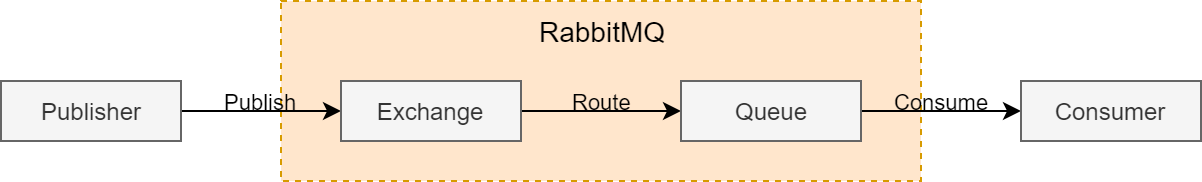
\includegraphics[width=\textwidth, height=0.9\textheight, keepaspectratio]{RabbitMQ_AMQP.png}
	\caption{RabbitMQ communication flow}
	\label{img:rabbitmqamqp}
\end{figure}

\paragraph{STOMP plugin}

As the name suggests, \acf{STOMP} is a simple protocol where messages are sent in frames.
A frame is a text message consisting of a command, an optional header and an optional body.
\ac{STOMP} requires a underlying 2-way streaming network protocol to send frames between client and server.
The communication flow is shown in Figure ~\ref{img:rabbitmqstomp}.
A client can be either a consumer or a publisher.
In both cases, the client only needs to know the connection information of the server for setup.
Unlike \ac{AMQP}, where the client also defines exchanges and queues, \ac{STOMP} requires that the logic is defined in the server.
The clients cannot define the routing behavior of the server, so the server must provide this logic.
To route a message, the server can use anything within it \cite{.25.09.2015}.
The RabbitMQ implementation of \ac{STOMP} has several routing options and each is provided by a separate destination.
To send a message to a specific destination, a \textit{destination string} can be used \cite[p. 191]{Roy.2018}.

\begin{figure}
	\centering
	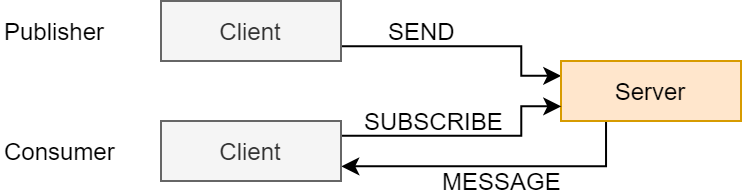
\includegraphics[width=\textwidth, height=0.9\textheight, keepaspectratio]{RabbitMQ_STOMP.png}
	\caption{RabbitMQ communication flow using STOMP}
	\label{img:rabbitmqstomp}
\end{figure}

\paragraph{MQTT plugin}

\ac{MQTT} is located between \ac{STOMP} and \ac{AMQP} from a functionality point of view.
It provides a basic routing like the \ac{AMQP} topic exchange shown in Figure ~\ref{img:rabbitmqmqtt}.
A client can publish a message on a topic (shown in Figure ~\ref{img:rabbitmqmqtt} with topic \textit{cat1/top1} and \textit{cat1/top2}).
A client can also subscribe to topics.
This is shown in Figure \ref{img:rabbitmqmqtt}, where \textit{Subscriber B} subscribes to both topics and therefore receives messages from both topics.
As with \ac{AMQP} topic exchange, the messages are copied and sent to each subscriber \cite[p.~4ff.]{Hillar.2017}\cite{AndrewBanks.2014}.
Finally, each message contains a \acf{QoS} attribute that determines how the message is handled in case of errors \cite{AndrewBanks.2014}.

\begin{figure}
	\centering
	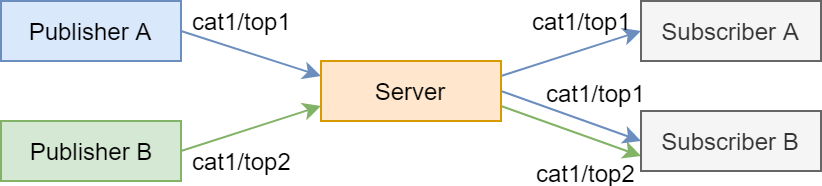
\includegraphics[width=\textwidth, height=0.9\textheight, keepaspectratio]{RabbitMQ_MQTT.png}
	\caption{RabbitMQ communication flow using MQTT}
	\label{img:rabbitmqmqtt}
\end{figure}

\paragraph{Protocol selection}

RabbitMQ can be used in several ways because it supports three protocols.
Consequently, the question remains which protocol to use.
In general, it is advisable to use a protocol that is already supported by an environment.
Another point to consider are the required communication features.
\ac{AMQP} is feature-rich, which can be too complicated for some application environments.
It also has a high latency, which can be a problem for unreliable networking of mobile devices \cite[p. 177]{Roy.2018}.
As described above, \ac{MQTT} has fewer features than \ac{AMQP} and \ac{STOMP} is even more lightweight than \ac{MQTT} \cite[p. 189]{Roy.2018}.
When deciding which protocol to use, it is also helpful to consider other projects.
For example, \ac{MQTT} is often used for \ac{IoT} applications.
This is probably due to the small code footprint or its suitability for low-bandwidth environments \cite[p. 178]{Roy.2018}\cite{AndrewBanks.2014}.
When using \ac{STOMP} the big advantage is that messages are sent in human-readable form (text based), but this is also a disadvantage.
\ac{AMQP} and \ac{MQTT} are binary and therefore more efficient than \ac{STOMP} in transmitting data.
Finally, it is important to mention that the \ac{STOMP} plugin for RabbitMQ adds an overhead, because RabbitMQ uses proxied \ac{AMQP} connections to communicate the translated \ac{STOMP} data \cite[p. 200]{Roy.2018}.

\paragraph{Conclusion}

RabbitMQ is very flexible because it supports several standard protocols, allowing for future technology exchanges.
Which protocol should be used depends on many factors, as described above.
Finally, some important factors that support RabbitMQ for the election, based of the persona needs.

RabbitMQ keeps messages in \ac{RAM} if possible and only when the \ac{RAM} is full, the messages are moved into memory.
To ensure good performance, additional nodes can be added to a running cluster, allowing dynamic scaling.
To ensure availability, nodes can be replicated and the message acknowledgment provides a delivery guarantee.
Another easy to implement feature in RabbitMQ is \textit{multicast}, which can be achieved via a fanout exchange \cite[p.~230ff.]{Dobbelaere.2017}.

\subsection{NATS}\label{cha:Technologies:communication:nats}

The \acf{NATS} is a communication technology that follows the \textit{publish-subscribe} pattern.
Its core objectives are simplicity, performance, and reliability \cite[p.~8]{Quevedo.2018}.
Communication is session-based and a session starts and ends with a connection.
When a session is closed, no data is persisted \cite[p.~3]{Quevedo.2018}.
\ac{NATS} is a non-binary transmission and only provides an \textit{at-most-once} \ac{QoS} when transmitting data \cite[p.~20]{Quevedo.2018}.
There is another popular project called \textit{NATS Streaming}, which adds an abstraction layer over \ac{NATS} and provides an \textit{at-least-once} \ac{QoS} \cite[p.~10f.]{Quevedo.2018}.
It also does not persist or buffer information by default, making it a true \textit{fire and forget} system \cite[p.~8]{Quevedo.2018}.

\ac{NATS} supports the subscription models \textit{fan-out} and \textit{queue subscription}.
Fan-out is the default, and it works like the \ac{AMQP} fanout exchange, but it still uses the subject (or topic in the \ac{AMQP} context).
So, any client that subscribes to a subject will receive all messages in that subject \cite[p.~6]{Quevedo.2018}.
Subjects can be divided into namespaces with a "." (\textit{period}).
A Subscription can be more general by using wildcards, such as "*" (\textit{asterisk}) for partial or token match and ">" (\textit{greater}) for full wildcard \cite[p.~31]{Quevedo.2018}.
Figure \ref{img:natspubsub} shows an example of fan-out communication with multiple clients and namespaces:
\textit{Client C} only receives the message from \textit{Client A}, because it has subscribed the topic \textit{data.test}, whereas \textit{Client D} receives every message published to a subject which starts with the namespace \textit{data}.
Therefore, it receives both messages.

\begin{figure}
	\centering
	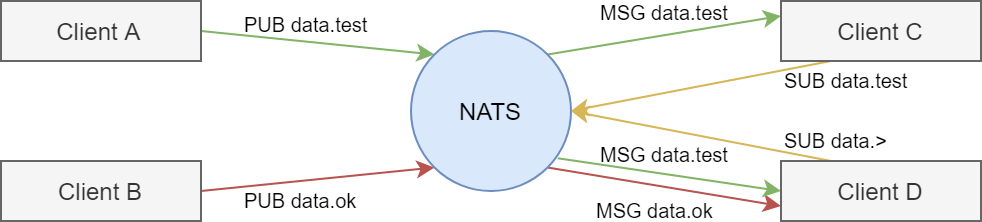
\includegraphics[width=\textwidth, height=0.9\textheight, keepaspectratio]{NATS_Fanout.png}
	\caption{NATS publish subscribe example}
	\label{img:natspubsub}
\end{figure}

The other subscription model \textit{queue subscription} works like \ac{AMQP} \textit{direct exchange}.
When a message is published to a subject, it is distributed to only one subscriber, instead of all.
The two subscription modes can be combined \cite[p.~34ff.]{Quevedo.2018}.
For example, a subject has two clients (\textit{A} and \textit{B}), which are subscribed via a \textit{queue subscription} and one client (\textit{C}) via a \textit{fan-out}.
Then clients \textit{A} and \textit{B} receive messages alternately and \textit{C} receives each message.

A powerful technique of \ac{NATS} is the \textit{request-response} pattern, which enables a completely asynchronous implementation.
An example is shown in Figure \ref{img:natsreqres}, where \textit{Client B} sends a request and \textit{Client A} responds.
This can be archived when \textit{Client B} provides a response subject and its name is passed along with the request.
So, \textit{Client A} knows where to publish the response \cite[p.~38ff.]{Quevedo.2018}.

The Request-Response pattern can be further improved if necessary, by reducing the latency.
To achieve this, \textit{Client A} must be replicated and \textit{Client B} must unsubscribe the response subject, once a message has been retrieved.
It is important that \textit{Client A} and its replicas use the \textit{fan-out} subscription model and the response subject should be unique to avoid collisions.
The result of this approach is that many responses are wasted because only the fastest respond is used.
However, if the main concern is time, this technique allows even faster responses.
Therefore it is called \textit{Lowest Latency Response} \cite[p.~40f.]{Quevedo.2018}.

\begin{figure}
	\centering
	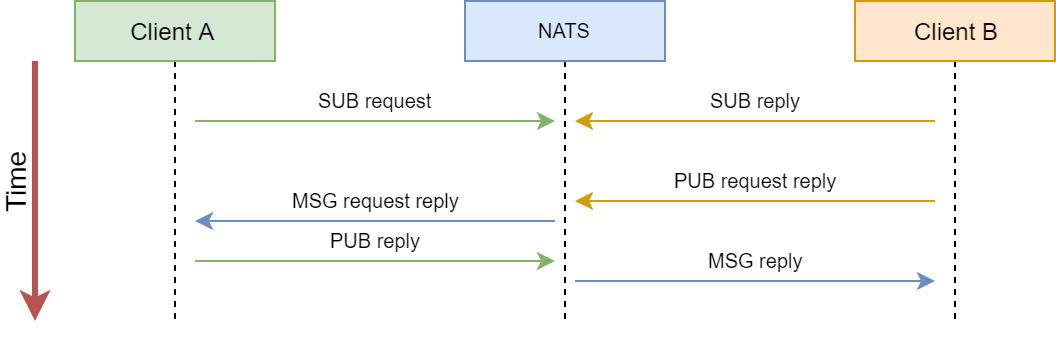
\includegraphics[width=\textwidth, height=0.9\textheight, keepaspectratio]{NATS_request_response.png}
	\caption{NATS request response example}
	\label{img:natsreqres}
\end{figure}

After considering the functionality of \ac{NATS}, the next step is to evaluate it based on the requirements of the personas.
One of the core objectives of \ac{NATS} is performance \cite[p.~8]{Quevedo.2018} and this is illustrated in a benchmark.
For example, in a benchmark comparison between \textit{NATS Streaming} and \textit{Apache Kafka}, \textit{NATS Streaming} was faster in almost every test \cite{TylerTreat.2016}.
It is important to note that \textit{NATS Streaming} uses \ac{NATS} in the core and adds an abstraction layer above it.
This indicates that \ac{NATS} is even faster than shown in the benchmark.
Another important factor is scalability and \ac{NATS} provides a high availability support via a clustering mode that is set up as a full-mesh of servers \cite[p.~8]{Quevedo.2018}.
Another key objective is simplicity \cite[p.~8]{Quevedo.2018}, which is represented by the relatively simple command set.
However, these allow powerful combinations such as mixing of subscription modes \cite[p.~35f.]{Quevedo.2018} and the \textit{Lowest Latency Response} technique \cite[p.~40f.]{Quevedo.2018}.
An important factor to consider is that \ac{NATS} core provides the \textit{at-most-once} \ac{QoS}.
This can be extended to \textit{at-least-once} using the \textit{NATS Streaming} project \cite[p.~10f.]{Quevedo.2018}.
After all, \ac{NATS} tries to stay alive at all costs.
This means that in case of a client connection that accumulates too much data without emptying it, the \ac{NATS} server will disconnect from the client to protect itself \cite[p.~9]{Quevedo.2018}.

\subsection{Apache Kafka}\label{cha:Technologies:communication:kafka}

Apache Kafka (in the following only \textit{Kafka}) is a log-based distributed streaming platform and offers high availability, storage and linear scale-out \cite[p.~14]{Stopford.2018}.
For fault tolerance and linear scale-out, the data is distributed across many machines \cite[p.~17f.]{Stopford.2018}.
\textit{Kafka} is suitable for a variety of applications, but before describing them, it is important to explain how \textit{Kafka} works.

Like the other asynchronous communication technologies, \textit{Kafka} follows the \textit{publish-subscribe} pattern.
This means that a client can publish a message to a topic, and a subscribed consumer receives the message.
In \textit{Kafka}, a message is treated like a log, which means that it is immutable and added to a message log.
The topics are divided into partitions \cite[p.~30]{Kumar.2017}, and each partition has its own message log \cite[p.~33]{Kumar.2017}.
To determine which message is routed to which partition, the message key is used \cite[p.~41]{Kumar.2017}.
To ensure high availability, topic partitions are replicated, where one partition is the leading partition and the others are the following partitions.
If the leader fails, a new leader is selected from the followers \cite[p.~33]{Kumar.2017}.

Partitions and their replicas are distributed among several brokers \cite[p.~17]{Stopford.2018}, and a broker can only have one or two partitions of the same topic.
A \textit{Kafka} cluster consists of several nodes, which in turn have several brokers \cite[p.~27]{Kumar.2017}.
This combination allows \textit{Kafka} to scale particularly well, so that it is no problem to have 100 nodes or even more \cite[p.~20]{Stopford.2018}.

The next important part of \textit{Kafka} is \textit{Zookeeper}.
It is responsible for several tasks, and without it \textit{Kafka} would not work.
For example, \textit{Zookeeper} takes care of the broker states, because broker do not persist their state \cite[p.~27]{Kumar.2017}\cite[p.~37f.]{Kumar.2017}.
\textit{Zookeeper} also knows the distributed locations of the partition leaders and followers \cite[p.~34]{Kumar.2017}.

A client who sends messages to a topic is called a producer, and a client who receives messages is called a consumer.
Each consumer belongs to a consumer group, and a consumer group can consist of several consumers \cite[p.~36f.]{Kumar.2017}.
Within a consumer group, only one consumer can be assigned to a topic partition.
This limits the degree of parallelism in a single consumer group \cite[p.~30f]{Kumar.2017}.
To publish or subscribe to a topic, the publishers or consumer needs to know which topic partition is relevant for them.
This means that a message is published or consumed directly from a topic partition, rather than from a topic.
Publishing or consuming a message is only possible from a topic partition leader \cite[p.~33]{Kumar.2017}\cite[p.~36]{Kumar.2017}.

All the parts described are combined in the Figure \ref{img:kafkacomflow}, where an example communication is shown.
The actual message transmission is only a small part, and a lot of work is done beside it.
In addition, the described communication flow shows the standard behavior, which can be changed.

Before any communication can take place, \textit{Zookeeper} must collect information about the locations of the topic partition (\textit{1}).
This information is then distributed to the producers and consumers (\textit{2}).
Now the producer knows the destination for the message and sends it to the lead partition \textit{A} (\textit{3}).
Partition \textit{A} stores the message and then informs \textit{Zookeeper} and the publisher about the successful writing (\textit{4}).
\textit{Zookeeper} then informs the consumer about a new message that is available (\textit{5}).
Now consumer \textit{A} can read the new message (\textit{6}) and updates its state at \textit{Zookeeper} (\textit{7}).

\begin{figure}
	\centering
	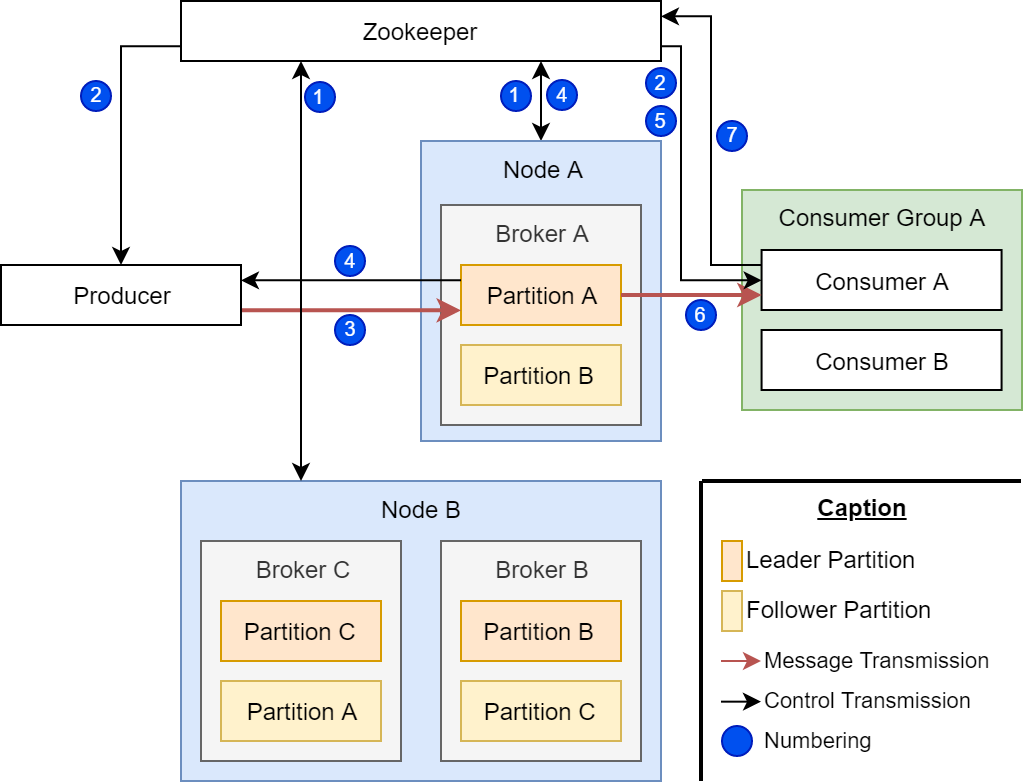
\includegraphics[width=\textwidth, height=0.9\textheight, keepaspectratio]{kafka_communication_flow.png}
	\caption{Kafka communication flow}
	\label{img:kafkacomflow}
\end{figure}

The last important part to complete \textit{Kafka}'s explanation is the message log within a partition.
Publishing a message to a message log within a partition involves several steps.
The process is shown in Figure \ref{img:kafkapubmsg}.
After a leading partition receives a message, it calculates the message offset, which is the identifier of a message within a partition.
The message is then appended to the message log, but not committed \cite[p.~18]{Stopford.2018}.
In addition, the message is sent to all its partition followers.
Each follower partition replies with an acknowledgment, and once everyone has responded, the message is committed to the message log.
The final step is to inform the producer that the message has been accepted and the \textit{Zookeeper} that a new message is available \cite[p.~36]{Kumar.2017}.

\begin{figure}
	\centering
	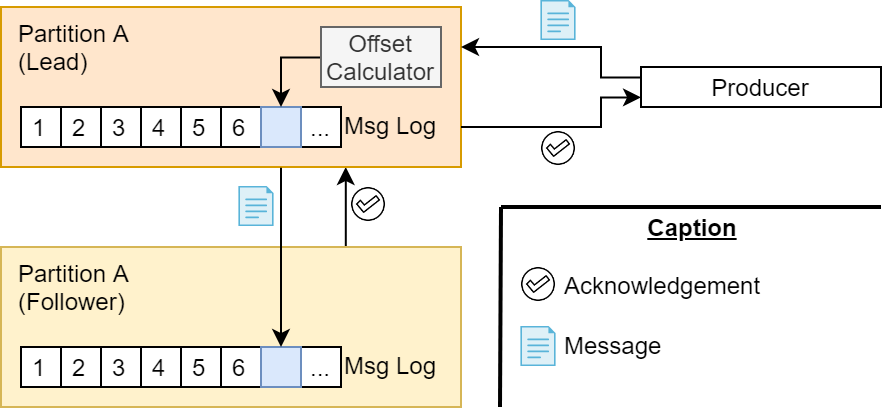
\includegraphics[width=\textwidth, height=0.9\textheight, keepaspectratio]{kafka_publish_message.png}
	\caption{Kafka publish message example}
	\label{img:kafkapubmsg}
\end{figure}

After explaining \textit{Kafka} and the concepts on which it is based, the open question arises as to what \textit{Kafka} is good for.
\textit{Kafka} can be used as a messaging system, which has already been described in the above communication example.
This includes the two traditional models of \textit{queue} and \textit{publish-subscribe}.
Queuing is realized by having multiple consumers within a consumer group.
Messages from a topic can only be consumed by one consumer within a consumer group.
There is an important side effect that the maximum number of consumers within a group is equal to the number of topic partitions.
On the other hand, \textit{publish-subscribe} is handled in such a way that several consumer groups can listen to the same topic.
In this way, each consumer group receives a published message.

Another specialty of \textit{Kafka} is its storage system.
Published messages are stored on disk, and Kafka’s disk structure enables good performance even when terabytes of data are stored.
The messages can be re-consumed as needed, making \textit{Kafka} a distributed file system for special purposes, designed for high performance, low-latency and replication.
The last feature of \textit{Kafka} is its ability to process data streams.
\textit{Kafka} provides a \textit{Streams API} that can consume and process messages from one topic and publish them to another topic.
This is very flexible because it uses the same interfaces as the actual producers and consumers \cite{ApacheKafka.01.06.2020}.

This concludes the general structure and major characteristics of \textit{Kafka}, but there are more features that are explained in \cite{Stopford.2018} and \cite{Kumar.2017}.
For example, an important feature that should be considered here is the message order guarantee.
\textit{Kafka}s default settings only guarantee message order within a partition.
It can be extended to guarantee the order within a topic or even globally, but this is associated with a high-performance overhead \cite[p.~30]{Kumar.2017}.
Another important fact is that \textit{Event Sourcing} architecture fits perfectly with \textit{Kafka}, since it can store messages like a database and replay the message log at any time.
Even if \textit{Kafka} is complex under the hood, it is still quite easy to use.
There are some quality of live features, such as not having to worry about queue depth and that slow consuming messages do not affect performance, which makes \textit{Kafka} easier the use.
\textit{Kafka}'s unique architecture allows for high speed reading of messaged.
Messages can be sent directly from storage because they are immutable logs.
As described at the beginning, \textit{Kafka} scales with virtually no limitations.
Finally, it offers countermeasures for denial of service attacks with a feature called \textit{quotas} \cite[p.~18ff.]{Stopford.2018}.
